\begin{figure}[t]
\centering
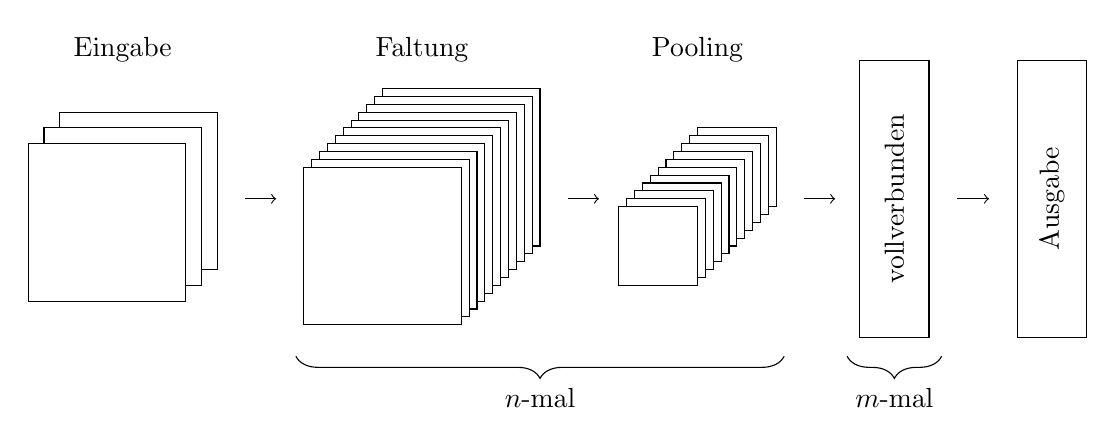
\begin{tikzpicture}
  \tikzstyle{node}=[rectangle, draw, minimum width=100pt, minimum height=25pt, inner sep=0pt, fill=white, rotate=90]
  \tikzstyle{rect}=[rectangle, draw, fill=white]
  \tikzstyle{path}=[->, shorten >= 10pt, shorten <= 10pt]

  % Eingabe.
  \draw[rect] (-0.1, 0.4) rectangle (1.9, 2.4);
  \draw[rect] (-0.3, 0.2) rectangle (1.7, 2.2);
  \draw[rect] (-0.5, 0)   rectangle (1.5, 2);

  % Faltung.
  \draw[rect] (4,   0.7)  rectangle (6,   2.7);
  \draw[rect] (3.9, 0.6)  rectangle (5.9, 2.6);
  \draw[rect] (3.8, 0.5)  rectangle (5.8, 2.5);
  \draw[rect] (3.7, 0.4)  rectangle (5.7, 2.4);
  \draw[rect] (3.6, 0.3)  rectangle (5.6, 2.3);
  \draw[rect] (3.5, 0.2)  rectangle (5.5, 2.2);
  \draw[rect] (3.4, 0.1)  rectangle (5.4, 2.1);
  \draw[rect] (3.3, 0)    rectangle (5.3, 2);
  \draw[rect] (3.2, -0.1) rectangle (5.2, 1.9);
  \draw[rect] (3.1, -0.2) rectangle (5.1, 1.8);
  \draw[rect] (3,   -0.3) rectangle (5, 1.7);

  % Pooling.
  \draw[rect] (8,   1.2) rectangle (9,   2.2);
  \draw[rect] (7.9, 1.1) rectangle (8.9, 2.1);
  \draw[rect] (7.8, 1)   rectangle (8.8, 2);
  \draw[rect] (7.7, 0.9) rectangle (8.7, 1.9);
  \draw[rect] (7.6, 0.8) rectangle (8.6, 1.8);
  \draw[rect] (7.5, 0.7) rectangle (8.5, 1.7);
  \draw[rect] (7.4, 0.6) rectangle (8.4, 1.6);
  \draw[rect] (7.3, 0.5) rectangle (8.3, 1.5);
  \draw[rect] (7.2, 0.4) rectangle (8.2, 1.4);
  \draw[rect] (7.1, 0.3) rectangle (8.1, 1.3);
  \draw[rect] (7,   0.2) rectangle (8,   1.2);

  \node at (0.7, 3.2) {Eingabe};
  \node at (4.5, 3.2) {Faltung};
  \node at (8,   3.2) {Pooling};

  \node[node] (1)  at (10.5, 1.3) {vollverbunden};
  \node[node] (2)  at (12.5, 1.3) {Ausgabe};

  \path[path] (1.9, 1.3) edge (3,    1.3);
  \path[path] (6, 1.3)   edge (7.1,  1.3);
  \path[path] (9, 1.3)   edge (10.1, 1.3);

  \path[path] (1) edge (2);

  \draw [decoration={brace,mirror,amplitude=8pt},decorate,-] (2.9,-0.7) -- node[below=8pt] {$n$-mal} (9.1,-0.7);
  \draw [decoration={brace,mirror,amplitude=8pt},decorate,-] (9.9,-0.7) -- node[below=8pt] {$m$-mal} (11.1,-0.7);
\end{tikzpicture}
  \caption[Netzarchitektur eines \glspl{CNN}]{Typische Netzarchitektur eines \glspl{CNN} bestehend aus beliebig vielen Faltungs- gefolgt von Poolingschichten.
  Die Abflachung der Merkmalskarten zu einem Vektor erlaubt die Verwendung beliebig vieler vollverbundener Schichten hin zur Ausgabe.}
\label{fig:cnn_aufbau}
\end{figure}
